\chapter{Suites infinies de variables aléatoires}
\sloppy


Soit $(\Omega, \mathcal{F}, P)$ un espace de probabilité.
\section{Modes de convergence}
Soit $(X_n)_{n \in \mathbb{N}}$ une suite de variables aléatoires (v.a.) définies sur $(\Omega, \mathcal{F}, P)$. Soit également $X$ une v.a. supplémentaire définie sur $(\Omega, \mathcal{F}, P)$.
\begin{definition}[Convergence presque sûre]
La suite $(X_n)_{n \in \mathbb{N}}$ converge presque sûrement vers $X$, ce que l'on note $X_n \xrightarrow{p.s.} X$, si
\[
P(\{\omega \in \Omega : \lim_{n \to \infty} X_n(\omega) = X(\omega)\}) = 1.
\]
\end{definition}
\begin{definition}[Convergence en moyenne d'ordre r ($L^r$)]
Soit $r \geq 1$. La suite $(X_n)_{n \in \mathbb{N}}$ converge vers $X$ dans $L^r(\Omega, P)$, ce que l'on note $X_n \xrightarrow{L^r} X$, si
\[
\lim_{n \to \infty} \mathbb{E}[|X_n - X|^r] = 0.
\]
\end{definition}
\begin{definition}[Convergence en probabilité]
La suite $(X_n)_{n \in \mathbb{N}}$ converge vers $X$ en probabilité, ce que l'on note $X_n \xrightarrow{P} X$, si
\[
\forall \varepsilon > 0, \quad \lim_{n \to \infty} P(|X_n - X| > \varepsilon) = 0.
\]
\end{definition}
\section{Liens entre convergences}
La convergence la plus difficile à établir est la convergence presque sûre.
\begin{proposition}
Si $X_n \xrightarrow{p.s.} X$, alors $X_n \xrightarrow{P} X$.
\end{proposition}
\begin{proof}
Supposons $X_n \xrightarrow{p.s.} X$. Par définition, cela signifie que $P(\{\omega \in \Omega : \lim_{n \to \infty} X_n(\omega) = X(\omega)\}) = 1$.
La définition de la limite d'une suite est :
\[
\lim_{n \to \infty} X_n(\omega) = X(\omega) \iff \forall \varepsilon > 0, \exists N \in \mathbb{N}, \forall n > N, |X_n(\omega) - X(\omega)| < \varepsilon.
\]
Pour des raisons de mesurabilité, on restreint $\varepsilon$ aux rationnels positifs, ce qui est suffisant.
\begin{align*}
    P(\lim_{n \to \infty} X_n = X) = 1 &\iff P\left(\forall \varepsilon \in \mathbb{Q}_+^*, \exists N \in \mathbb{N}, \forall n > N, |X_n - X| < \varepsilon\right) = 1 \\
    &\iff P\left(\bigcap_{\varepsilon \in \mathbb{Q}_+^*} \bigcup_{N \in \mathbb{N}} \bigcap_{n > N} \{|X_n - X| < \varepsilon\}\right) = 1
\end{align*}
Puisqu'il s'agit d'une intersection dénombrable d'événements de probabilité 1, chacun de ces événements doit avoir une probabilité de 1.
\[
\implies \forall \varepsilon > 0, \quad P\left(\bigcup_{N \in \mathbb{N}} \bigcap_{n > N} \{|X_n - X| < \varepsilon\}\right) = 1
\]
En passant au complémentaire, la probabilité devient 0 :
\[
\forall \varepsilon > 0, \quad P\left(\left(\bigcup_{N \in \mathbb{N}} \bigcap_{n > N} \{|X_n - X| < \varepsilon\}\right)^c\right) = P\left(\bigcap_{N \in \mathbb{N}} \bigcup_{n > N} \{|X_n - X| \geq \varepsilon\}\right) = 0
\]
Posons $A_N = \bigcup_{n > N} \{|X_n - X| \geq \varepsilon\}$. La suite d'événements $(A_N)_{N \in \mathbb{N}}$ est décroissante. Par continuité de la mesure de probabilité pour les suites décroissantes, on a :
\[
P\left(\bigcap_{N \in \mathbb{N}} A_N\right) = \lim_{N \to \infty} P(A_N) = \lim_{N \to \infty} P\left(\bigcup_{n > N} \{|X_n - X| \geq \varepsilon\}\right) = 0.
\]
Or, pour tout $N$, on a l'inclusion $\{|X_N - X| \geq \varepsilon\} \subset \bigcup_{n > N} \{|X_n - X| \geq \varepsilon\}$.
Donc, $P(|X_N - X| \geq \varepsilon) \leq P(\bigcup_{n > N} \{|X_n - X| \geq \varepsilon\})$. En passant à la limite quand $N \to \infty$, on obtient:
\[
\forall \varepsilon > 0, \quad \lim_{N \to \infty} P(|X_N - X| \geq \varepsilon) = 0.
\]
Ceci est la définition de la convergence en probabilité, $X_n \xrightarrow{P} X$.
\end{proof}
\begin{proposition}
Soit $r \geq 1$. Si $X_n \xrightarrow{L^r} X$, alors $X_n \xrightarrow{P} X$.
\end{proposition}
\begin{proof}
Soit $\varepsilon > 0$. On utilise l'inégalité de Markov. Écrivons :
\begin{align*}
    \mathbb{E}[|X_n - X|^r] &= \int_{\Omega} |X_n - X|^r dP \\
    &= \int_{\{|X_n - X| \geq \varepsilon\}} |X_n - X|^r dP + \int_{\{|X_n - X| < \varepsilon\}} |X_n - X|^r dP \\
    &\geq \int_{\{|X_n - X| \geq \varepsilon\}} |X_n - X|^r dP \\
    &\geq \int_{\{|X_n - X| \geq \varepsilon\}} \varepsilon^r dP = \varepsilon^r P(|X_n - X| \geq \varepsilon).
\end{align*}
D'où l'on tire:
\[
P(|X_n - X| > \varepsilon) \leq \frac{1}{\varepsilon^r} \mathbb{E}[|X_n - X|^r].
\]
Comme $X_n \xrightarrow{L^r} X$, on a $\lim_{n \to \infty} \mathbb{E}[|X_n - X|^r] = 0$. Par conséquent,
\[
\lim_{n \to \infty} P(|X_n - X| > \varepsilon) = 0,
\]
ce qui prouve que $X_n \xrightarrow{P} X$.
\end{proof}
\begin{proposition}[Compatibilité avec l'addition]
Si $X_n \xrightarrow{*} X$ et $Y_n \xrightarrow{*} Y$, alors $X_n + Y_n \xrightarrow{*} X+Y$, où $*$ peut être la convergence p.s., $L^r$ (avec le même $r \ge 1$), ou en probabilité.
\end{proposition}
\begin{proof}[Indication pour la convergence en probabilité]
On utilise l'inégalité triangulaire et la sous-additivité de la probabilité. Pour tout $\varepsilon > 0$:
\[
\{|(X_n+Y_n) - (X+Y)| > \varepsilon\} \subset \{|X_n-X| + |Y_n-Y| > \varepsilon\} \subset \{|X_n-X| > \varepsilon/2\} \cup \{|Y_n-Y| > \varepsilon/2\}.
\]
D'où,
\[
P(|(X_n+Y_n) - (X+Y)| > \varepsilon) \leq P(|X_n-X| > \varepsilon/2) + P(|Y_n-Y| > \varepsilon/2).
\]
Chacun des termes de droite tend vers 0 lorsque $n \to \infty$.
\end{proof}
Nous pouvons également traduire dans le langage des v.a. les théorèmes classiques de théorie de la mesure.
\begin{example}[Théorème de convergence dominée]
Soit $(X_n)$ une suite de v.a. telle que :
\begin{enumerate}
    \item Il existe une v.a. $X$ telle que $X_n \xrightarrow{p.s.} X$.
    \item Il existe une v.a. $Y \geq 0$ intégrable ($\mathbb{E}[Y] < \infty$) telle que $|X_n| \leq Y$ p.s. pour tout $n$.
\end{enumerate}
Alors $X_n \xrightarrow{L^1} X$, et en particulier, $\lim_{n \to \infty} \mathbb{E}[X_n] = \mathbb{E}[X]$.
\end{example}
\section{Exemples}
On se place sur l'espace de probabilité $(\Omega, \mathcal{F}, P) = ([0,1], \mathcal{B}([0,1]), \lambda_{|[0,1]})$, où $\lambda$ est la mesure de Lebesgue.
\begin{example}
Considérons la suite de fonctions définie par $X_{2k}(\omega) = \mathbf{1}_{[0, 1/2]}(\omega)$ et $X_{2k+1}(\omega) = \mathbf{1}_{[1/2, 1]}(\omega)$ pour $k \in \mathbb{N}$.
Pour tout $\omega \in [0,1]$, la suite $(X_n(\omega))$ oscille entre 0 et 1 (sauf en $\omega=1/2$) et ne converge donc pas. Cette suite ne converge en aucun sens (p.s., $L^r$, ou P).
\begin{figure}[H]
\centering
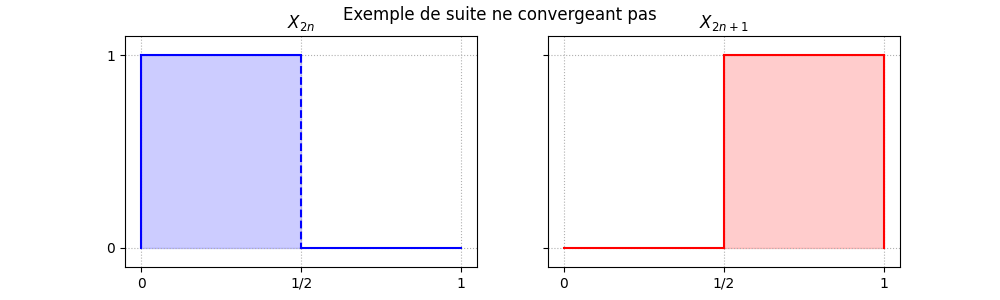
\includegraphics[width=0.7\textwidth]{ex3_plot1.png}
\caption{Suite $(X_n)$ qui n'admet aucune limite.}
\label{fig:ex1_noconv}
\end{figure}
\end{example}
\begin{example}[La suite "machine à écrire"]
Considérons la suite de v.a. $(X_n)$ qui sont des indicatrices d'intervalles qui balaient $[0,1]$ avec une largeur qui tend vers 0. Par exemple :
$X_1 = \mathbf{1}_{[0,1]}$, $X_2 = \mathbf{1}_{[0,1/2]}$, $X_3 = \mathbf{1}_{[1/2,1]}$, $X_4 = \mathbf{1}_{[0,1/3]}$, etc.
Cette suite converge en probabilité vers 0, car la mesure (longueur) de l'intervalle où $X_n=1$ tend vers 0.
\[
P(|X_n - 0| > \varepsilon) = P(X_n=1) \to 0 \quad \text{pour } 0 < \varepsilon < 1.
\]
Cependant, pour tout $\omega \in [0,1]$, la suite $X_n(\omega)$ prend la valeur 1 une infinité de fois. Donc $\limsup_{n \to \infty} X_n(\omega) = 1$, tandis que $\liminf_{n \to \infty} X_n(\omega) = 0$. La limite ponctuelle n'existe pas, donc la suite ne converge pas presque sûrement.
On a donc $X_n \xrightarrow{P} 0$ mais $X_n \not\xrightarrow{p.s.} 0$.
\begin{figure}[H]
\centering
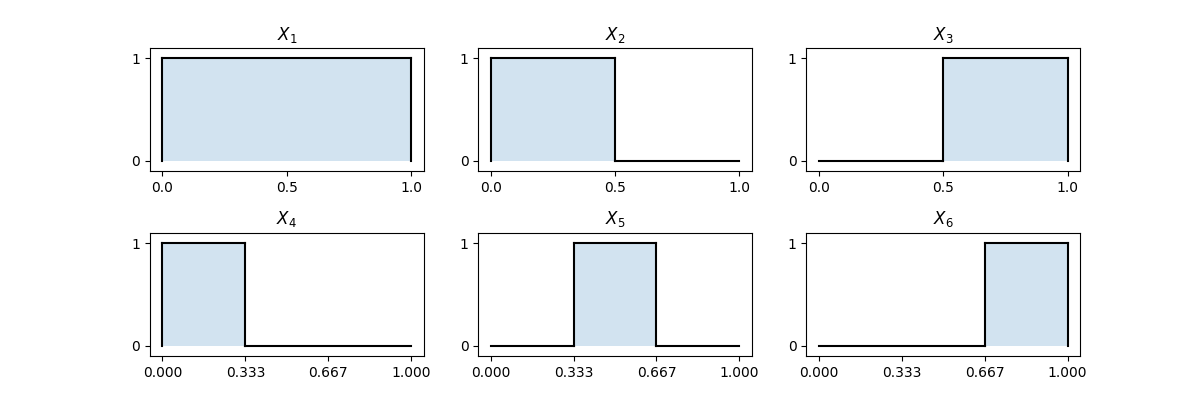
\includegraphics[width=\textwidth]{ex3_plot2.png}
\caption{Les premiers termes de la suite "machine à écrire".}
\label{fig:typewriter}
\end{figure}
\end{example}
\section{Indépendance pour une suite infinie}
\begin{definition}
Une suite infinie de tribus $(\mathcal{F}_n)_{n \in \mathbb{N}}$ est dite indépendante (resp. d'événements, de v.a.) si toute famille finie extraite de la suite est indépendante.
\end{definition}
\begin{remark}
Il y a une analogie avec la notion de liberté en algèbre linéaire.
\end{remark}
\begin{theorem}[Regroupement par blocs infinis]
Soit $(X_n)_{n \in \mathbb{N}}$ une suite de v.a. indépendantes. Soit $(I_k)_{k \in \mathbb{N}}$ une partition de $\mathbb{N}$ (des parties deux à deux disjointes dont la réunion est $\mathbb{N}$). Alors les tribus $\mathcal{J}_k = \sigma(X_n, n \in I_k)$ pour $k \in \mathbb{N}$ sont indépendantes.
\end{theorem}
\section{Le modèle analytique pour le jeu de pile ou face}
Nous voulons construire un espace de probabilité $(\Omega, \mathcal{F}, P)$ sur lequel est définie une suite de v.a. $(X_n)_{n \in \mathbb{N}^*}$ de loi de Bernoulli symétrique sur $\{-1, 1\}$ (parfois appelée loi de Rademacher), et qui sont toutes indépendantes.
Nous prenons $(\Omega, \mathcal{F}, P) = ([0,1], \mathcal{B}([0,1]), \lambda)$, la mesure de Lebesgue sur $[0,1]$.
À un nombre réel $\omega \in [0,1[$, nous associons son développement dyadique (binaire) unique, celui qui ne se termine pas par une suite infinie de 1 :
\[
\omega = \sum_{n=1}^\infty \frac{\omega_n}{2^n}, \quad \text{où } \omega_n \in \{0, 1\}.
\]
Nous définissons alors, pour $n \geq 1$, la suite de variables aléatoires $(X_n)$ par :
\[
\forall \omega \in [0,1[, \quad X_n(\omega) = 2\omega_n - 1 \in \{-1, 1\}.
\]
Ces fonctions sont appelées les fonctions de Rademacher. On peut montrer que cette suite $(X_n)$ répond à la question.
Par exemple, $X_1(\omega) = 1$ si $\omega_1=1$ (i.e., $\omega \in [1/2, 1[$) et $X_1(\omega) = -1$ si $\omega_1=0$ (i.e., $\omega \in [0, 1/2[$).
De manière générale, l'ensemble $X_n^{-1}(\{1\})$ est l'union de $2^{n-1}$ intervalles dyadiques de longueur $1/2^n$. La mesure totale de cet ensemble est donc $2^{n-1} \times \frac{1}{2^n} = \frac{1}{2}$.
D'où $P(X_n = 1) = \lambda(\{\omega: X_n(\omega) = 1\}) = \frac{1}{2}$, et de même $P(X_n = -1) = \frac{1}{2}$.
\begin{figure}[H]
\centering
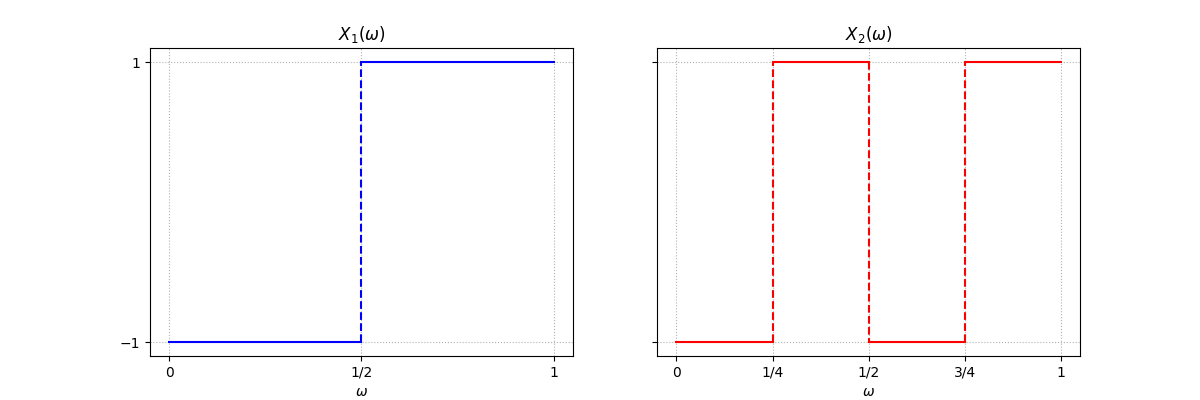
\includegraphics[width=0.8\textwidth]{rademacher_plots.png}
\caption{Les deux premières fonctions de Rademacher.}
\label{fig:rademacher}
\end{figure}
Pour montrer que les $(X_n)_{n \geq 1}$ sont indépendantes, il suffit de montrer que pour tous $\varepsilon_1, \dots, \varepsilon_n \in \{-1, 1\}$, on a $P(X_1=\varepsilon_1, \dots, X_n=\varepsilon_n) = \prod_{i=1}^n P(X_i=\varepsilon_i)$.
\begin{align*}
    P(X_1=\varepsilon_1, \dots, X_n=\varepsilon_n) &= \lambda(\{\omega \in [0,1[ : \forall i \in \{1..n\}, X_i(\omega)=\varepsilon_i\}) \\
    &= \lambda(\{\omega \in [0,1[ : \forall i \in \{1..n\}, \omega_i = \frac{1+\varepsilon_i}{2}\})
\end{align*}
L'ensemble des $\omega$ dont les $n$ premiers chiffres binaires sont fixés forme un intervalle dyadique de longueur $1/2^n$. Par exemple, si $\varepsilon_1=1, \varepsilon_2=-1$, on cherche les $\omega$ avec $\omega_1=1, \omega_2=0$, c'est-à-dire $\omega \in [0.10_2, 0.11_2) = [1/2, 3/4[$. La longueur est $1/4 = 1/2^2$.
Donc, $P(X_1=\varepsilon_1, \dots, X_n=\varepsilon_n) = \frac{1}{2^n}$.
Comme $P(X_i=\varepsilon_i) = 1/2$ pour tout $i$, on a bien $\prod_{i=1}^n P(X_i=\varepsilon_i) = (\frac{1}{2})^n$.
Les variables sont donc indépendantes. Nous possédons une suite infinie de "pièces" indépendantes.
\section{Marche aléatoire sur les entiers}
On modélise une marche aléatoire symétrique sur $\mathbb{Z}$.
\begin{itemize}
    \item La marche démarre en 0.
    \item À chaque étape, on lance une pièce équilibrée.
    \item Pile : on fait un pas de +1 (à droite). Face : on fait un pas de -1 (à gauche).
    \item On réitère l'opération à partir de la nouvelle position.
\end{itemize}
Notons $S_n$ la position du marcheur après $n$ pas. Formellement :
\[
S_0 = 0, \quad S_n = X_1 + X_2 + \dots + X_n,
\]
où les $(X_i)$ sont une suite de v.a. i.i.d. avec $P(X_i=1)=P(X_i=-1)=1/2$.
\begin{center}
"Allumeur" \quad $\longleftrightarrow$ \quad 0 \quad $\longleftrightarrow$ \quad "Réverbère"
\end{center}
Une question naturelle est : quelle est la probabilité que le marcheur repasse un jour par son point de départ (le "réverbère original")? On cherche donc à calculer :
\[
P(\exists n \in \mathbb{N}^*, S_n = 0) = P\left(\bigcup_{n=1}^\infty \{S_n=0\}\right).
\]
Pour que $S_n=0$, il faut autant de pas +1 que de pas -1. Le nombre total de pas $n$ doit donc être pair. Posons $n=2k$.
On calcule d'abord la probabilité de revenir en 0 après $2k$ pas.
Soit $\alpha$ le nombre de pas +1 et $\beta$ le nombre de pas -1. On doit avoir $\alpha+\beta=2k$ et $\alpha-\beta=0$, ce qui implique $\alpha=\beta=k$.
Le nombre de chemins de longueur $2k$ revenant à l'origine est le nombre de façons de choisir les $k$ pas +1 parmi les $2k$ pas, soit $\binom{2k}{k}$. Le nombre total de chemins possibles de longueur $2k$ est $2^{2k}$.
D'où,
\[
P(S_{2k}=0) = \frac{\binom{2k}{k}}{2^{2k}}.
\]
En utilisant l'approximation de Stirling, $m! \sim \sqrt{2\pi m} (m/e)^m$, on trouve :
\[
P(S_{2k}=0) \approx \frac{1}{\sqrt{\pi k}} \quad \text{pour } k \to \infty.
\]
La probabilité de revenir à l'origine à un instant donné tend vers 0.
\begin{figure}[H]
\centering
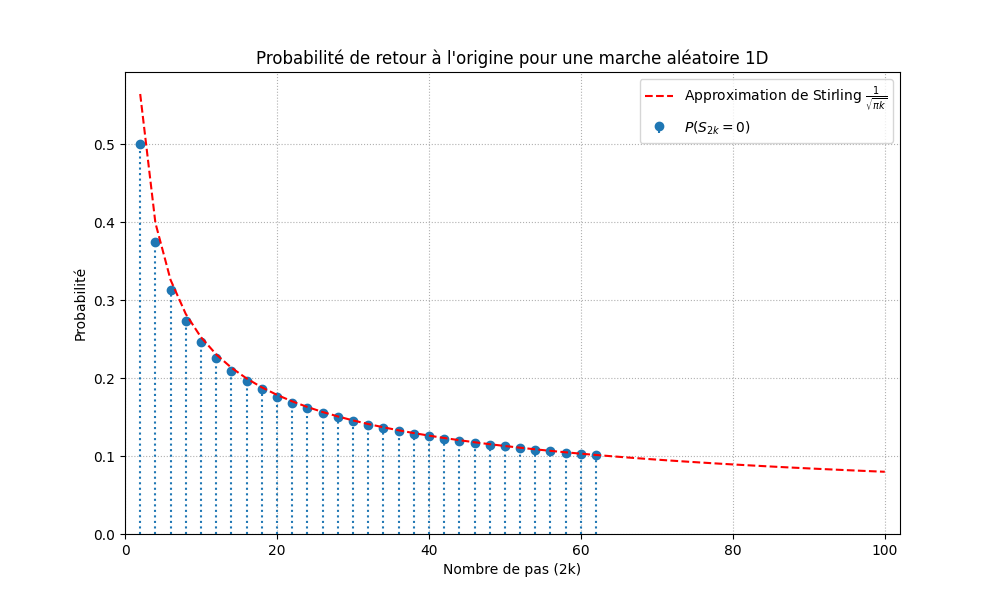
\includegraphics[width=0.8\textwidth]{proba_return_zero.png}
\caption{Évolution de $P(S_{2k}=0)$ en fonction du nombre de pas.}
\label{fig:return_prob}
\end{figure}
Pour calculer la probabilité de revenir \emph{un jour}, on décompose l'événement en une union d'événements disjoints : le premier retour à l'origine. Soit $f_{2k} = P(S_2 \neq 0, \dots, S_{2k-2} \neq 0, S_{2k}=0)$.
La probabilité de revenir un jour est $\sum_{k=1}^\infty f_{2k}$.
\begin{lemma}
La probabilité de premier retour à l'instant $2k$ est liée à la probabilité de retour par la relation (non triviale) :
\[
f_{2k} = \frac{1}{2k-1} P(S_{2k}=0) \quad (\text{pour } k \ge 1).
\]
\end{lemma}
La probabilité de revenir un jour est donc $\sum_{k=1}^\infty f_{2k}$. Il se trouve que cette somme vaut 1.
\[
P(\exists n \in \mathbb{N}^*, S_n = 0) = \sum_{k=1}^\infty f_{2k} = 1.
\]
La marche aléatoire simple symétrique sur $\mathbb{Z}$ est donc \emph{récurrente} : elle est certaine de revenir à son point de départ.